\chapter{Methods}
\label{chapter:methods}
%TODO : Change logo
% \emph{[Supervised machine learning basics, neural networks, convolutional, fully connected layers, Recurrent NN, Model ensemble options (compare it with traditional alg.) ]}
% \bigskip

% JUHAA
% It feels to me that your methods section is somehow lacking the thread. Of course there was still missing parts but more clear connection to your implementation would help to understand it. And you need to explain only main methods you really use. I would try to avoid having short sub sub sections.

% What I try to say is that try to compress your text a bit and add clear links to your implementation. For example “this method is often used with problems that are very similar to the one discussed in the thesis…”


This chapter starts with a theoretical part related to machine learning and Artificial Neural Networks with the concept of Model Ensemble at the end. The theoretical concepts are always supported with typical use cases to help the reader better understand the different approaches.A supervised machine learning framework will be chosen to formulate a generalized model for occupancy detection based on the features extracted from the dataset described in the previous chapter. The presumption is, that by using nonlinear classification methods the speech information can be extracted with higher precision.


\section{Machine Learning introduction}

Machine learning as a subset of Artificial Intelligence research aims to develop algorithms, which performance improves with data given during the learning process. Or as famously known from Tom M. Mitchell: "Machine learning is the study of computer algorithms that allow computer programs to automatically improve through experience" or “A computer program is said to learn from experience E with respect to some class of tasks T and performance measure P, if its performance at tasks in T, as measured by P, improves with experience E” \cite{ML_book_Mitchell97}.

In the next section, the three main branches of machine learning will be introduced briefly, supervised, unsupervised, and reinforcement learning. 


\subsection{Types of Machine Learning tasks}


\subsubsection{Supervised Learning}

In a Supervised Learning setting a dataset is given with the corresponding correct output or so-called label for each example. Starting with a labeled dataset the tasks can be divided into two main categories: classification and regression. In the first case, the machine learning model tries to learn the generalized mapping between the input dataset and the provided labels or classes while in regression the model output is a continuous function \cite{DL_book_Goodfellow}.

\subsubsection{Unsupervised Learning}

Unsupervised learning algorithms aim to extract patterns from data without any a priori information provided such as labels or scores. In clustering, the patterns are used to group samples based on their similarity and, in addition, the clusters can help detecting outliers of a given dataset. The research field dedicated to outlier detection is called anomaly detection and their findings used extensively in several industrial scenarios, in finance for bank fraud detection or in cybersecurity domain for intrusion detection and system health monitoring \cite{DL_book_Goodfellow}. Alternatively, in principal component analysis, the extracted information is used to compress the training dataset by selecting the features which most discriminates the samples from each other and reduce the dimensionality of the problem \cite{DL_book_Goodfellow}.


\subsubsection{Reinforcement Learning}

Reinforcement learning problems are often modeled as for an agent to interact with an environment and take the best action sequence, which maximizes its reward \cite{RL_book_Sutton1998}. Explicit data collection is not needed for the problem in advance in the traditional sense, as the data is most often generated during the learning phase. One key challenge is that the agent has to find the right balance between exploration  of new actions and exploitation of already proven solutions. Board games such as chess and Go are the most recent areas where implementation of RL algorithms turned to be useful for reaching superhuman performance level strategies \cite{silver18alphazero}.

%JUHAA
% Reference for GO chess etc..
% https://discovery.ucl.ac.uk/id/eprint/10069050/1/alphazero_preprint.pdf

\subsubsection*{Discussion on the used approach}
Among the three introduced machine learning paradigm, for our goal, the easiest solution would be to form it as a Supervised Learning challenge. Collecting audio files representing unoccupied and occupied room scenarios and labeling them respectively, gives us a binary classification problem. Building a model aiming to spot the human speech or noises in a given time frame. Moreover, to ensure the usability of the model in various circumstances, the aim is to use the most diverse training sources, cover the most common use cases, and choosing the right architecture for the model, to be able to capture the underlying patterns in the dataset. While the concept of Unsupervised Learning would target to find anomalies or similarities in the dataset without human input, which might mislead the learning process since our target is clearly defined.


\section{Artificial Neural Networks}

Artificial Neural Networks \cite{DL_book_Goodfellow}, in the most general sense, are directed computational graphs with learnable parameters. Early models, such as the Perceptron, were inspired by the structure of the human brain, artificially replicating neurons as universal computational units and synapses to transmit signals across the network. Conventionally, neurons are grouped into layers which perform similar functionality, then layers stacked together to construct the final network.

The main incentive behind the research of Neural Networks is to define mathematical models which can adapt to the task requirements and perform better with experience. Feedforward architectures with nonlinear activation functions can approximate any continuous function according to the Universal Approximation theorem \cite{HORNIK1991univ}, which makes them viable for complex high dimensional problems with the right training algorithms.

\subsection{The Perceptron}

In machine learning, the Perceptron \cite{rosenblatt1958perceptron} was one of the first realizations of an Artificial Neuron, constituted of a weighted sum of its inputs plus the bias term which then forwarded to a thresholding function:


\begin{equation}
      f(x) =
    \begin{cases}
      1 & \text{if $W\cdot x + b > 0$}\\
      0 & \text{otherwise.}
    \end{cases} 
\end{equation}

The $f(x)$ function is an early version of the more complex activation functions used nowadays, it simply implements a step function, therefore the model will output 1 if $x$ was positive and 0 in negative cases. The decision boundary can be adjusted by the $b$ bias term. Therefore if used in single layer configuration it can only converge for linearly separable problems and require a custom training algorithm given that the activation function is not differentiable.

\begin{figure}[ht]
  \begin{center}
    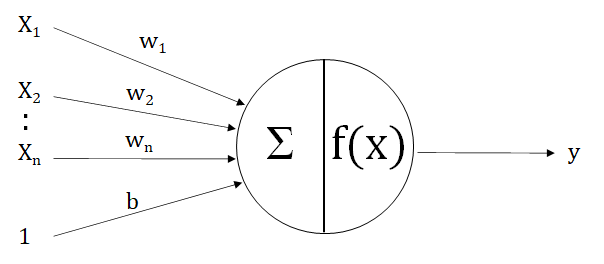
\includegraphics[width=0.7\textwidth]{thesistemplate/images/perc.png}
    \caption{Structural diagram of a Single Perceptron node.}
    \label{fig:perceptron_struct}
  \end{center}
\end{figure}


\subsection{Multi-Layer Perceptron}


In the Multi-Layer Perceptron model (MLP) perceptrons are organized into a layered structure where the input data flows only forward, from the input to the output, hence the alternative name, Feedforward Networks. Alternatively, in recurrent neural networks \cite{sutskever2013training_rnn}, the computation flow contains feedback loops, allowing the model to capture historical information, so the current prediction will not depend only on the current input but the preceding ones, too. It is widely applied to time series data forecasting and natural language processing tasks.

Single-layer Perceptrons can only find viable classification boundaries for linearly separable problems, for non-linearly separable more complex problems multiple-layer setup is needed. 

Neural networks are intended to approximate some ideal function $\hat f$, in the case of classification, $y = \hat f(x)$ where $x$ denotes the input and $y$ is the assigned category for $x$. An MLP aims to find this mapping $y = f(x, \theta)$ by adapting its parameters $\theta$ during the learning process \cite{DL_book_Goodfellow}.

% \begin{align*} 
% z &= W^T x,  \\     
% y  &= \sigma (z)
% \end{align*}

% JUHAA
% What is the reason for this equation, no link to the text

% also with (l) layer number marked in top

\subsection{Convolutional Neural Networks}

Convolutional neural networks (CNN) are a special type of feedforward network, where the weights are shared across the layer and each neuron is only connected to a subset of input elements determined by their locations. It has first gained popularity in Imagenet \cite{deng2009imagenet} Large Scale Visual Recognition challenge for image classification acting as a feature extractor usually in the first part of the network. Stacking several Convolutional layers with nonlinear activation functions together allows the network to extract high-level or abstract information from an image in an automated way, by finding the best low-level features and combining them for the final prediction.

Convolutional Networks can be thought of as feedforward networks that apply convolution instead of matrix multiplication \cite{DL_book_Goodfellow}. The function takes two arguments, the previous layer output as input and a kernel, and outputs a feature map. The kernel is usually one-dimensional for time series data and 2D for image data. The kernel parameters are adapted by the learning algorithm during training. \autoref{fig:cnn_parshare} illustrates the effect of the application of a kernel instead of the dense connections.

Nodes are only connected to the closest ones in the previous layer determined by the kernel size, in contrast to MLP structure where every all of the nodes are connected between two layers. Moreover, instead of learning the weights for each node-node connection, we are sharing the kernel parameters across the layer. Most implementations compute several feature maps with different kernels on the same input, therefore increasing the output tensor dimensions.


\begin{figure}[ht!]
  \begin{center}
    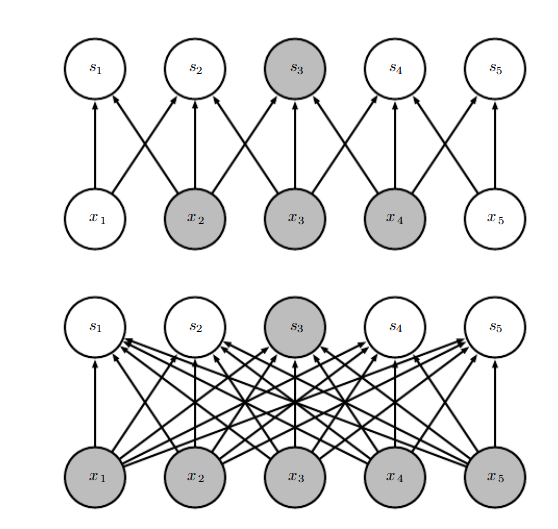
\includegraphics[width=0.5\textwidth]{thesistemplate/images/cnn_sparse.png}
    \caption{Comparison of Convolutional (upper) and Fully connected (lower) layers for parameter sharing, sparse connection is illustrated with arrows and gray coloring on the nodes \cite{DL_book_Goodfellow}.}
    \label{fig:cnn_parshare}
  \end{center}
\end{figure}


The first breakthrough happened in the late 1990s when deep learning had proven to be useful for handwritten character recognition tasks, with a relatively simple 5 layered structure involving only 2 convolutional layers for feature extraction \cite{lecun1998CNN}.

% \begin{itemize}
%     \item TODO: Kernel size, stride, padding image
%     \item TODO: Pooling explanation, max, average
% \end{itemize}

\subsection{Activation functions}

Activation functions as a nonlinear transformation play an important role in Multi-layer neural network modeling. Any combination of linear functions would remain a linear function, so to model nonlinear processes we need to employ nonlinear transformation in the computation \cite{nwankpa2018activation}. Another criteria from a computational point of view is differentiability since for automated learning the gradient must be computed using back-propagation. 

Some of the most commonly used activation functions are visible on \autoref{fig:act_func}. Sigmoid or Logistic function restricts the output to [0,1] interval with the formula given below, which are often used for last layers to output probability. Tanh or hyperbolic tangent exhibits similar characteristics in shape but transforms the input to range [-1,1] symmetrically. However, these functions are subject to the vanishing gradient problem, making the gradient-based learning slow due to the almost zero gradient outside the transitioning middle part. So if the system starts or ends up in those flat sections the parameter updates might be slow and ineffective without additional tricks such as momentum update \cite{QIAN1999145momentum}.

Rectified Linear Unit or shortly ReLU is the most widely used activation function currently, it mitigates the vanishing gradient problem for positive numbers because its gradient is always 1 for every positive input. Even if the gradient is undefined in zero, practical implementations usually substitute f'(0) = 0, which reduces the computational complexity with its simple definition. Further developed solutions includes Leaky ReLU \cite{DBLP:leakyReLU} and  Exponential Linear Unit ELU \cite{clevert2015fast_elu}, as an attempt to allow the learning for negative inputs.

\begin{equation}
    \mathrm{Sigmoid}(x) = \frac{1}{1 + \exp(-x)}
\end{equation}

\begin{equation}
    \mathrm{Tanh}(x) = \frac{\exp(x) - \exp(-x) }{\exp(x) + \exp(-x)}
\end{equation}

\begin{equation}
    \mathrm{ReLU}(x) = max(0,x)
\end{equation}

\begin{figure}[ht]
  \begin{center}
    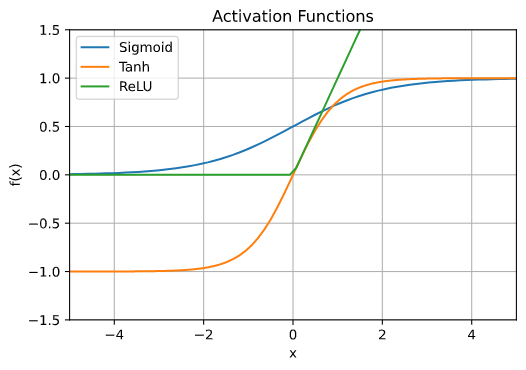
\includegraphics[width=0.58\textwidth]{thesistemplate/fig/activation_funcs.png}
    \caption{Most commonly used activation functions.}
    \label{fig:act_func}
  \end{center}
\end{figure}


% \section{Training techniques}

\section{Regularization techniques}

%JUHAA
% Consider, if you want to use these sub-sub-sub sections. You could have regularization topic only.

This section provides a general overview of the most common methods and concepts for achieving high accuracy values for a supervised machine learning problem. Regularization is a set of tools aiming to reduce the testing error by preventing overfitting the model on the training dataset.

\subsection{Dropout}
The dropout layer randomly sets some of the input tensor elements to zero with a predefined probability $p$ during the training process, which has proven to be useful for avoiding overfitting in various situations \cite{dropout_effect}.
%JUHAA
% Give at least one example

The reason behind eliminating part of the neuron outputs during the learning process is to force to build a more generalized model which is robust even in extreme conditions and helps the neurons to form generalized learning instead of specializing only to recognize one feature.
% https://arxiv.org/pdf/1207.0580.pdf

\subsection{Batch normalization}

%JUHAAA
% Picture with names of the parts of the process would help understanding where normalization takes its place.

A Batch normalization (BN) layer normalizes the output of a layer in a mini-batches during training, as a part of the network structure. Allows having larger learning rates, a more stable training process and reduced dependence on initialization \cite{ioffe2015batch}.

It is usually applied after a fully connected or convolutional layer and before the activation function for maximal efficiency.
%https://arxiv.org/pdf/1502.03167.pdf


% \subsection{Non-Convex Optimization}

% Cross-entropy loss: for binary classification
% \begin{equation}
%     L(x,y) = - \Big[ y\log(x) + (1-y)\log(1-x) \Big],
% \end{equation}
% where $x$ denotes the model output, while $y$ represents the target.

% Backpropagation: is a nonlinear optimization method for minimising the loss function by updating the parameters of the neural network.

% contents:
% \begin{itemize}
%     \item loss functions, binary cross-entropy in our case
%     \item backpropagation
%     \item gradient descent, momentum    %https://arxiv.org/abs/1609.04747   -   An overview of gradient descent optimization algorithms
%     \item optimizers, Adam \cite{kingma2017adam}
% \end{itemize}


\section{Model Ensemble}

% \emph{[Theoretical intro, block diagram of the prediction model]}

The high-level concept of the multisensor presence detector is to find a viable framework and building blocks for synchronizing the different sensor inputs and extracted predictions into one unified room occupancy state. Our work is focusing on only binary classification, to differentiate between empty and occupied office meeting room scenarios. Although initial research suggests that from the analog audio and PIR signals more information could be inferred like crowd size, identification of participants age, mood, we leave that for future research options and discuss it more in detail in Chapter \ref{chapter:discussion}, because it is just partially related to our topic.

Choosing a model ensemble approach was an early architectural design decision influenced by multiple factors. Previous research reports deploying single supervised ML models on top of multidimensional data collected from different environmental sensors (see Section \ref{section:Multisensor_research}), but the data collection is usually restricted only to one office room. These datasets are inherently carrying the special usage behaviors of the workers together with the unique arrangement of sensors, which can be misleading for developing a general occupancy prediction model expected to work in multiple different scenarios. The research field is currently lacking a reliable and diverse training dataset covering multiple locations and sensory inputs. The problem is even more visible with the audio or noise level information. To make the model more robust we tried to aim to use as many training examples as possible, but selecting only the ones where both audio and PIR information is available for the same room we would have limited ourselves to recordings from our office exclusively. Therefore, models dedicated for audio and PIR were separately trained, and in a third block the predictions were merged into one final decision. A high level overview of the multi-model topology is reported in \autoref{fig:multisens_pred_proc}.

%JUHAA
% No reference for this image in the text
\begin{figure}[ht!]
  \begin{center}
    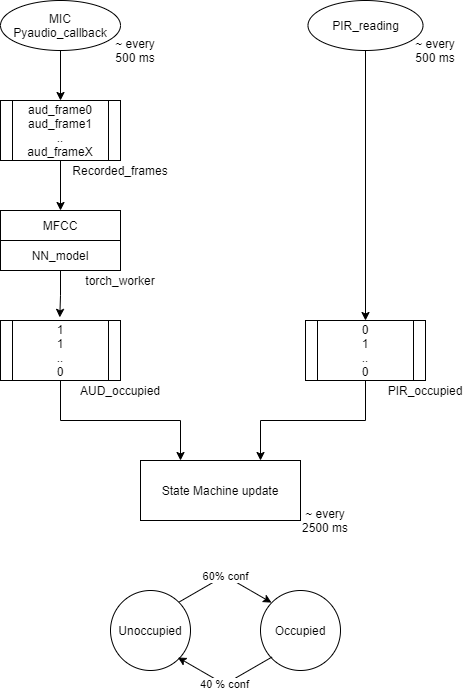
\includegraphics[width=0.58\textwidth]{thesistemplate/fig/multisensor_uml.png}
    \caption{Multisensor prediction process on the Raspberry Pi 4B platform.}
    \label{fig:multisens_pred_proc}
  \end{center}
\end{figure}

\section{Embedded AI development process}

Developing machine learning algorithms with embedded deployment generally imposes additional constraints on the process, due to the hard limitations of the selected hardware platform. An overview of the followed workflow can be seen in Figure \ref{fig:embAI_workflow} down below. As in most embedded AI projects, the dataset manipulation and neural network training steps are implemented in a regular desktop PC environment while the embedded platform is only used to run the inference with the already trained network parameters for testing purposes. In the next section, we will follow through each step to create a binary classification model for human presence detection based on sound. 

Starting with target selection, we present methods and design choices with reasoning for data collection and labeling. The careful selection of data sources is crucial for a positive outcome, it fundamentally defines and limits the theoretical capabilities of the model. In the preprocessing step we will generate the input for the training by windowing the audio signal and computing the selected MFCC features and reshaping them into a 2D matrix. This section is followed by several model training with grid search. The best-performing models which meet the computational limitations of the embedded platform get selected and converted to C arrays and libraries. Finally, the supporting functionality will be implemented which bridge the gap between the sensors and the machine learning model input, namely interfacing and feature extraction.



% https://arxiv.org/pdf/1911.03314.pdf

% TODO: change the line to model conversion to embedded platform
\begin{figure}[ht!]
  \begin{center}
    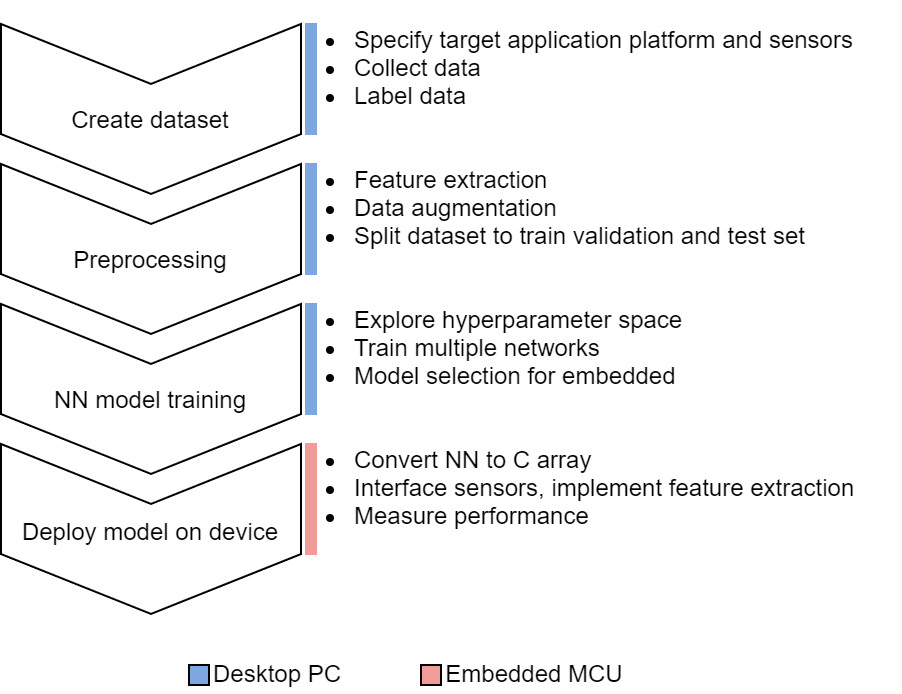
\includegraphics[width=0.75\textwidth]{thesistemplate/images/embAI_process.png}
    \caption{Embedded AI development workflow, adapted from \cite{wang2020fannonmcu}.}
    \label{fig:embAI_workflow}
  \end{center}
\end{figure}



%#################################################################################################################
%#################################################################################################################

\chapter{Audio based presence detection}

In this work, we had to make an arbitrary design decision early on, related to the focus of the ideal capabilities of the machine learning model, given the limited amount of computational resource for inference and helping the testing process, considering only the most typical use cases. Therefore our target is to recognize the human presence in the audio flow mostly based on speech and partially based on other additional noises such as placing and moving objects on a desk. 


By stating this early on the project will allow us to collect data to specifically cover these situations together with additional publicly available datasources, for a supervised machine learning classification setup.


%The audio sensors can pick up even the smallest noises in a silent room like keyboard typing or breathing as an indication of human presence, but in meeting rooms speech is the easiest marker to detect due to the relative loudness compare to the background noise and the characteristic frequencies people use to communicate.

\section{Data collection and analysis}

A large, diversified dataset is essential for any kind of machine learning problem. Given our final goal to test and run the model in real-time on an embedded platform with a certain digital microphone, we have collected data also with the same hardware tools used in the implementation. Moreover, we have used subsets of large publicly available datasets for extending the training set, leading to a more generalized model. First, the data collection approach will be elaborated with special attention to the used hardware and environmental choices for recording. This will be followed by the external audio sources selected for training. Finally, a summary will close the section, where all the different audio files are categorized and grouped into a condensed table.

Given the problem definition, the desired behavior for the audio-based machine learning algorithm is to distinguish between human presence and empty room scenarios from the audio feed. This frames the task as a binary classification, and to construct a proper dataset we need to collect data for both cases and label them for the training.


\subsection{Field Data collection}

For easy and quick data collection on-site, we have utilized a Raspberry Pi 4B with the same MEMS microphone used in the implementation (see  \autoref{subsub:Aud_sensor}). Fortunately, the Raspberry Pi board can interface the audio mic with the same I2S bus as the microcontroller and with the help of well documented high-level libraries made the data collection and the initial model testing fairly convenient. All audio was recorded with 16kHz to match with the target for the implementation. 

In the case of an occupied room, we placed the setup into a relatively large open office space and recorded short pieces of conversation with the approval of the people present at that time. Usually, the recording equipment was placed at a desk in the middle of the room, while employees had a casual talk next to it. But due to the cumbersome process for requesting consent and often empty offices, most of the speech data was borrowed from external sources. The condensed speech recording sums up 10 minutes in total.

While for representing unoccupied rooms, the sensor was placed in various empty meeting rooms on-site with the purpose to record not only the silence therefore the microphone inherent noise but also noises related to activities outside the examined room. These include environmental noises caused by wind, rain moreover attenuated speech, cars, or other noises coming through windows and closed doors. Additionally, a private apartment was used for collecting data representing environments with a higher background noise level. The apartment had windows open and closed while cars were passing by in front of it. Furthermore in random intervals construction noises made the recording more diverse due to renovation in the building. The manual recordings related to the empty room class altogether reach two hours in duration.


\begin{figure}[ht]
  \begin{center}
    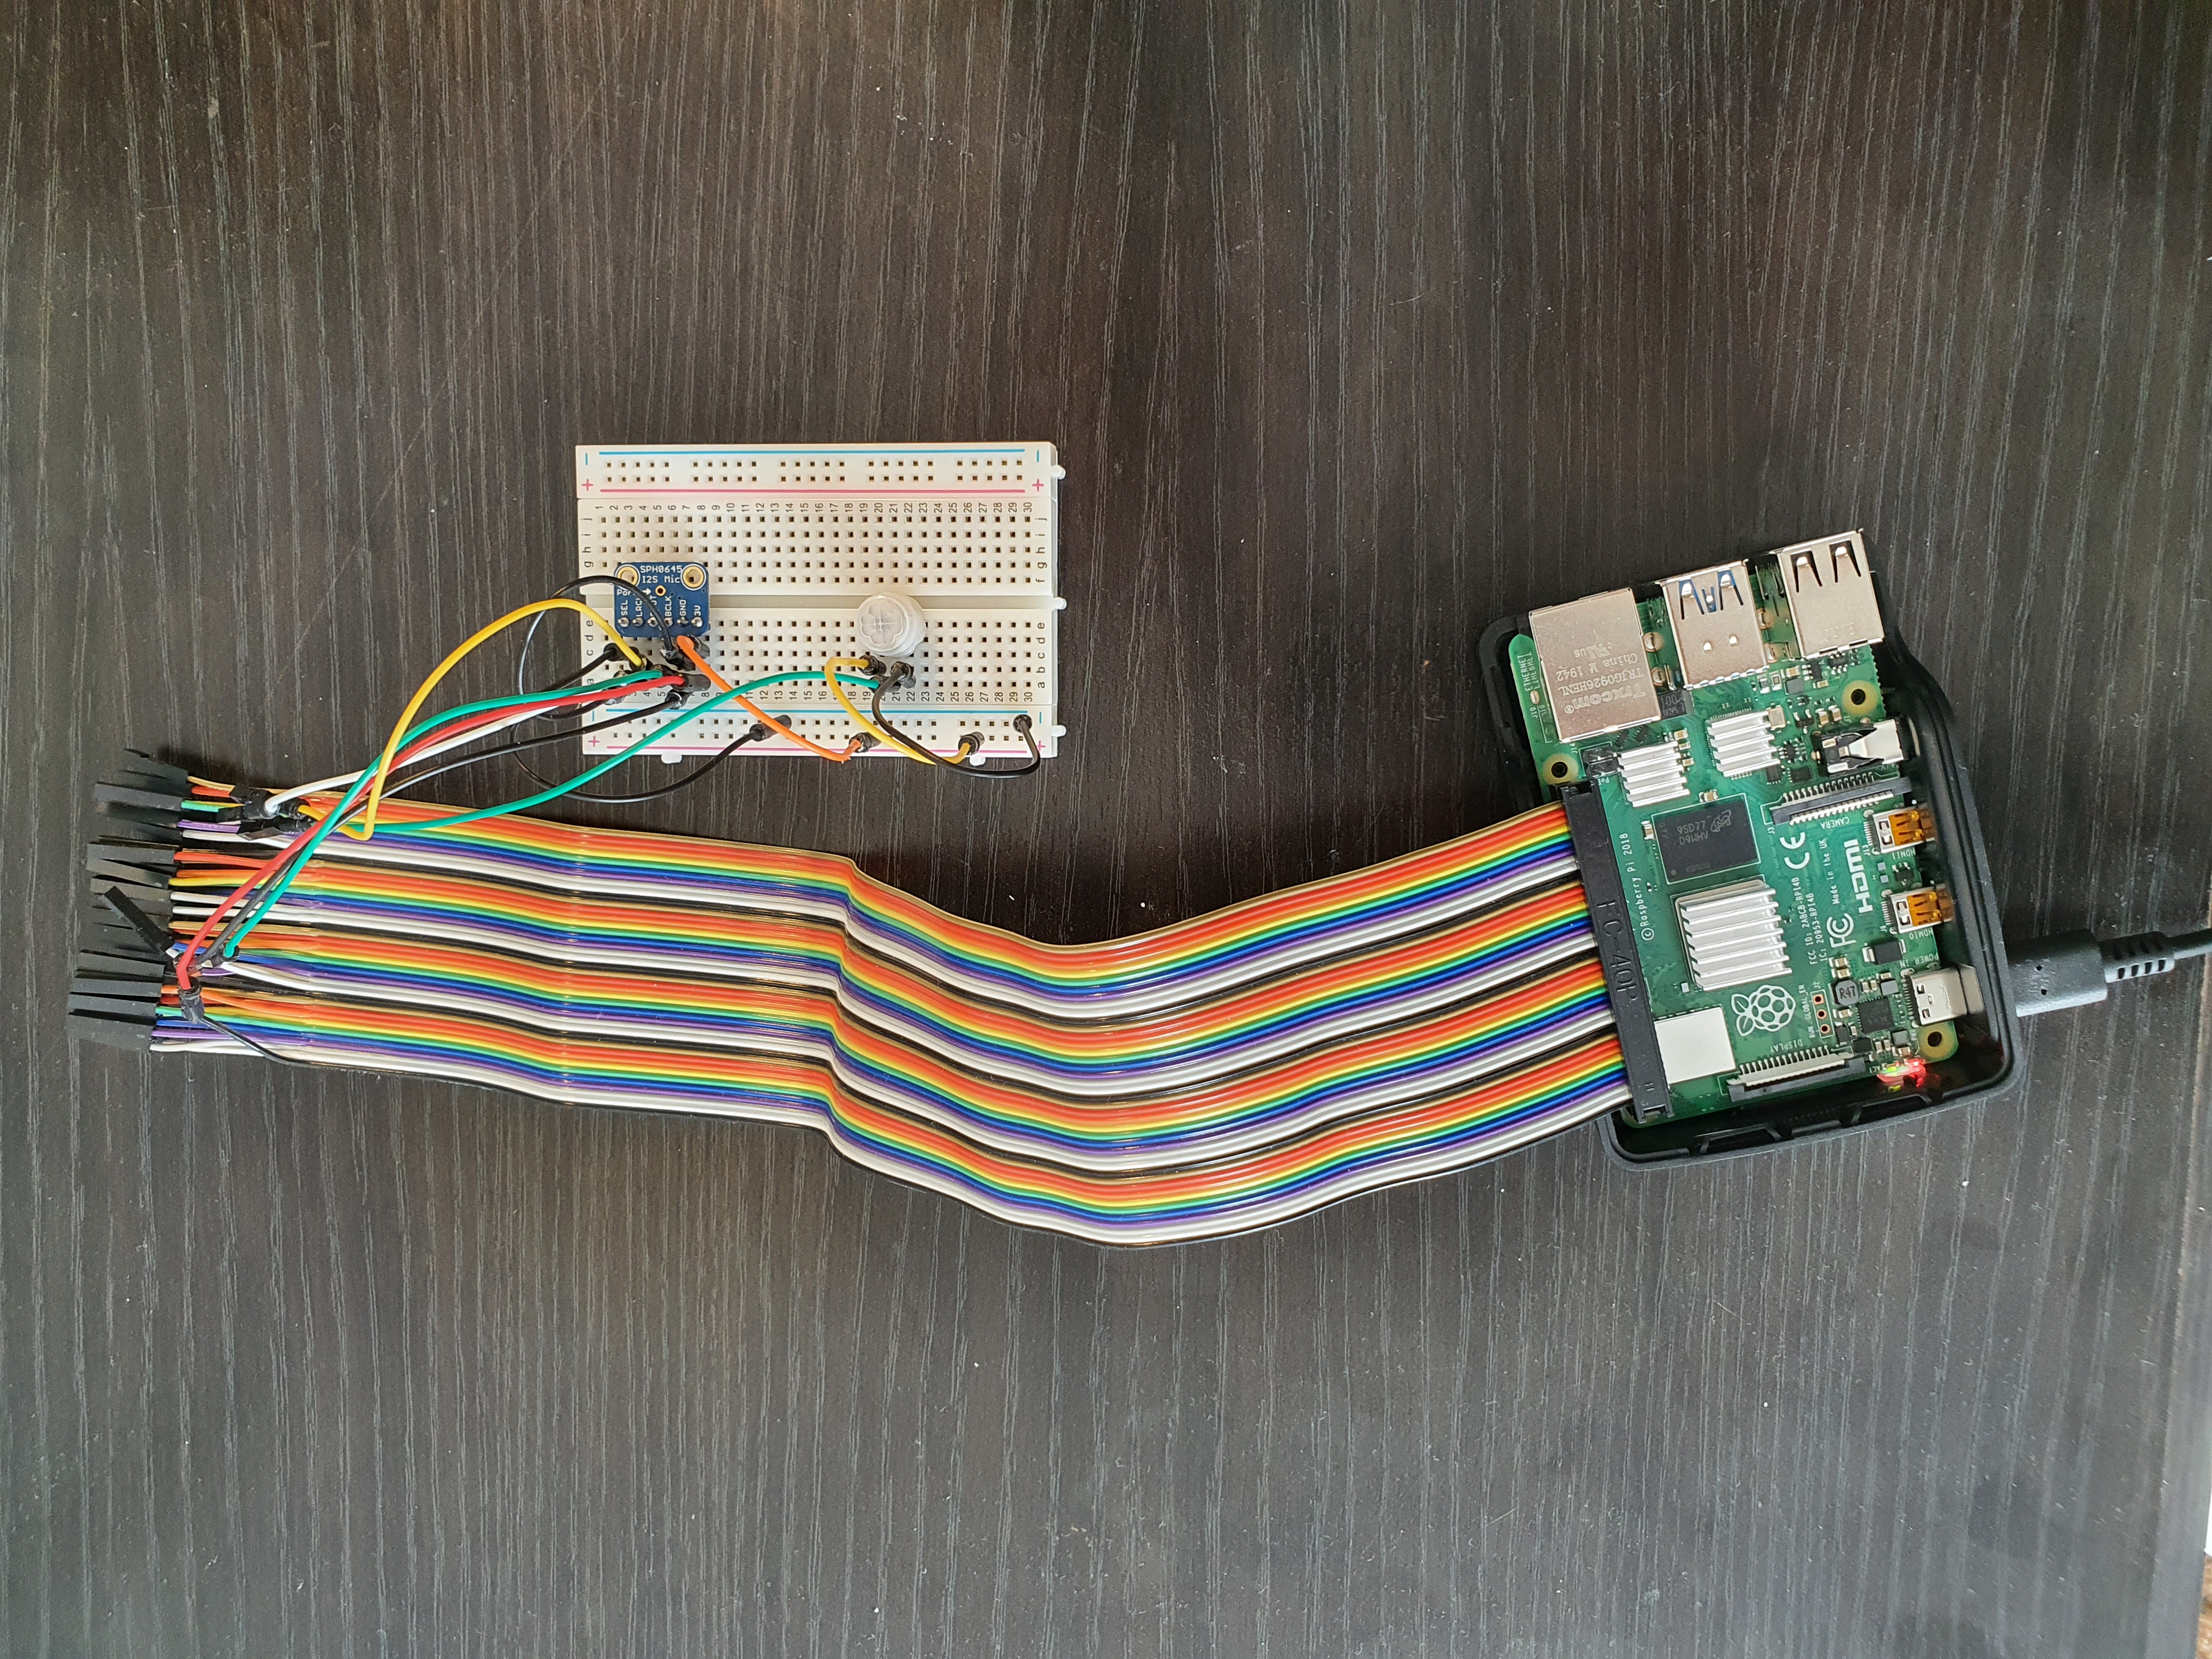
\includegraphics[width=0.6\textwidth]{thesistemplate/images/rpi_setup.jpg}
    \caption{Raspberry Pi 4B data collection setup with digital PIR and Sound sensors.}
    \label{fig:rpi_coll}
  \end{center}
\end{figure}

\subsection{External Data sources}

Since our aim is mostly voice activity detection, for that purpose many large, high quality, and diverse audio datasets are available for training purposes. During the selection process, our objective was to find human speech and background noises most similar to the test scenarios.

\paragraph*{Librispeech}\cite{librispch} is a publicly available corpus for Automatic Speech Recognition (ASR) derived from English audiobooks summing up to 1000 hours of speech by 2500 participants usually in background noise free environments. The audio is sampled at 16kHz and provided under the CC BY 4.0 license. Although the dataset is immense and the size is justified for speech recognition tasks we only used the dev-clean subset, a few hours of data produced by a total of 40 speakers. Clean refers to lower Word Error Rate (WER) speakers, meaning their speech was easier to decode with a baseline algorithm trained on WSJ (Wall Street Journal) dataset. Librispeech was used exclusively as a representation of occupied room state, can be viewed as a simulated conversation.

\paragraph*{QUT-NOISE} \cite{qut_noise} is a collection of background noises categorized into five different scenarios; CAFE, HOME, STREET, CAR, REVERB, in a total of 10 hours. After listening to short parts of each category, in the HOME segment, HOME-KITCHEN were selected as occupied room state, while CAR as unoccupied. HOME-KITCHEN as indicated in the title was recorded in a kitchen, during some sort of food preparation most probably. It was selected to make the learning more robust and able to spot non-speech-based human presence. In CAR scenario, researchers were collected street noise while driving, and it resembled most of the outdoor noises one would expect as background noise in a meeting room next to a street. All the samples were recorded at a 48 kHz sample rate and the data is publicly available under the CC-BY-SA license. The selected HOME recording is around 35 minutes long while the CAR scenario takes 130 minutes.


\paragraph*{Generated Noise} samples. Several noise samples were added to the training set simulating the self-noise of the selected microphone or monotonic noises present in indoor spaces produced by HVAC or other electronic devices. The selected noise profiles are white and red (Brownian) noise, after empirical testing of the perceived sound. White noise has approximately equal intensity across the different frequencies while red noise has the energy focused on longer wavelengths (smaller frequencies) and decreasing towards higher frequencies, analogously to the electromagnetic spectrum of the red light. A total of 35 minutes of sound was produced in this way.

% \begin{itemize}
%     \item Plot frequency spectrum of the white and the red noise if you really have too much free time
% \end{itemize}

\subsection{Summary of the training dataset}

 Overall, the whole constructed dataset consists of 12 hours of audio approximately. During the data collection, we paid special attention to represent the most typical use cases that might appear in an office environment while keeping the quantity of the two classes in balance. The different sources and their corresponding audio length are summarised in \autoref{tab:aud_database_sum} below.
\begin{table}[ht]
\centering
\begin{tabular}[t]{|l|l|r|}
\hline
\textbf{Category}           &   \textbf{Source}             & \textbf{Length (min:s)}\\
\hline
\multirow{4}{*}{Occupied}   &   Librispeech, dev-clean      &  323:16\\
                            &   QUT-Noise, home-kitchen     &   33:09\\
                            &   Open office (Rec.)          &   10:00\\
\cline{2-3}
                            &   \textbf{Total:}             &  \textbf{366:25}\\
\hline
\multirow{5}{*}{Unoccupied} &   QUT-Noise, car-window        &  130:56\\
                            &   Empty room (Rec.)           &   121:45\\
                            &   Air Conditioner noise       &   60:00\\
                            &   Generated noise             &   35:00\\
\cline{2-3}
                            &   \textbf{Total:}             &  \textbf{347:41}\\
\hline
\end{tabular}
\caption{Summary of the audio database.}
\label{tab:aud_database_sum}
\end{table}%




%Contents:
%\begin{itemize}
%  \item Data collection with Raspberry Pi 4B, time duration, empty meeting room, open office situations - ok
%  \item External audio souces, Librispeech \cite{librispch}, QUT-NOISE \cite{qut_noise}, white noise - ok, maybe ESC-50
%  \item reasoning about the 16k Sample Rate, previous studies, industry actors... - okayish
%  \item distribution of the dataset for training - ok
%\end{itemize}

% other audio datasets
% https://pytorch.org/audio/stable/datasets.html
% https://research.qut.edu.au/saivt/databases/qut-noise-databases-and-protocols/
% https://eprints.qut.edu.au/38144/1/c38144.pdf
% https://www.openslr.org/12
% https://commonvoice.mozilla.org/en



\section{Data loading and resampling}

As a first preparation step for data processing, we are loading each audio file to memory with a unified target sample rate of 16 kHz. A subset of the dataset was recorded with a different sampling rate, mostly with 48kHz, which needed to be filtered and resampled to the new target using a high-quality Kaiser window with 64 zero-crossings.
%https://resampy.readthedocs.io/en/0.1.5/api.html

The 16 kHz sampling rate and the Nyquist theorem imply that in our analysis the sampled signal can represent frequencies up to 8KHz correctly. The fastest and computationally most efficient VADs such as the Google WebRTC implementation uses only 8 kHz as a sampling frequency leaving them with only 4 kHz bandwidth for speech detection. However, apart from the resource-constrained implementations, higher sampling frequencies are leading to better results especially from a noise tolerance point of view. Moreover, human speech has frequency components higher than 4 kHz, and the richer representation could allow more sophisticated and robust behavior from the model.

% https://www.dpamicrophones.com/mic-university/facts-about-speech-intelligibility

After looking at the time series audio signal profiles, a relatively large offset can be observed in the signals recorded manually using the Raspberry Pi platform with the MEMS microphone. Regular recordings used from other sources do not have this feature. The phenomenon is due to the physical properties of the device (explained more in detail in \autoref{subsub:Aud_sensor}) and needs to be removed to reduce classification bias, not to mislead the training algorithm. Since all the recordings from the selected MEMS microphone have a constant DC offset, audio files were normalized to zero mean at this step, while in the embedded implementation a DC blocking filter will be applied (see \autoref{subsub:dc_blocking}).

% \begin{itemize}
%     \item TODO: Histogram on the time series data from mic and external, and after the DC was removed
% \end{itemize}

\section{Slicing and labeling}

In the slicing step, we need to determine the window size, which will be the basis of the feature extraction and directly influences the responsiveness of the final machine learning model in real-time inference, since we need to aggregate at least one window of data to calculate the features for prediction. Fixed input size is required for feed-forward neural networks hence the predetermined window size, and in the next steps, one set of extracted features corresponding to one windowed audio signal will be the basis for the model output.

All the data were sliced into 500 ms pieces with zero overlap, the label automatically added based on which category the audio file belonged to during data collection. As an industry-standard most VAD systems are operating with 20-30 ms of audio for one prediction allowing one to experience instantaneous feedback given the low delay, but just long enough to determine the presence of speech. The however larger window size can lead to increased confidence in the prediction given that the system has more data to consider. The loss in the response time is not considered critical at this scale, since the delay timers controlling the luminaries have values in the range of 10-45 minutes. 

Loosen the requirements and increase the window size to 500 ms have an additional indirect benefit with regards to the training process. It makes the labeling easier, assuming that the speech data does not contain long pauses, which would mislead the training. In the case of the Librispeech, the audio was split in every situation when a silence longer than 300 ms were detected, aiming to divide the source into sentences, so the final training set does not contain long periods of silence. On the other hand for environmental noises, we do not face this issue since the sound profile is monotonic. 

\section{Feature extraction}

In the last preprocessing step before the neural network training, we are transforming the audio slices from the time domain to the frequency domain with the help of Short Term Fourier Transformation to finally get the set of MFCC features representing the signal. Starting from 500 ms of audio (8000 elements) an FFT with the size of 512 will create 16 spectrum sections each representing around 30 ms of audio. From each spectrum computed 21 Mel-frequency cepstral coefficients are extracted, from which the first one will get discarded, leaving a total of 20 by 16 elements matrix. \autoref{fig:mfcc_img_comp} shows one representative 2D array example for each class. The first MFCC feature has been discarded in many projects, it usually corresponds to the signal energy or DC component which we do not wish to embed in the model decision process. Human speech should be spotted regardless of the sound volume.

The number of MFCCs extracted varies greatly in recent research works, earlier solutions with lower sampling rates usually compute 9-13 features, while newer versions can go as high as 20 or 40. The area of use influences the design choice by great detail. In Environmental Scene Classification and Automatic Speech Recognition, given these problems are more complex than Voice Activity Detection, require more information, and often use a high sampling rate (48 kHz) with 40 MFCC sometimes combined with Delta and Delta-Delta features. Delta and Delta-Delta are the first and second derivatives of the MFCC series. Other, more primitive methods include Zero Crossing Rate (ZCR) and Short-Term Energy (STE) computation on the time-series signal but these approaches are generally performing poorly in noisy environments and cannot distinguish between different sound sources, only noise levels.


\begin{figure}[ht!]
  \begin{center}
    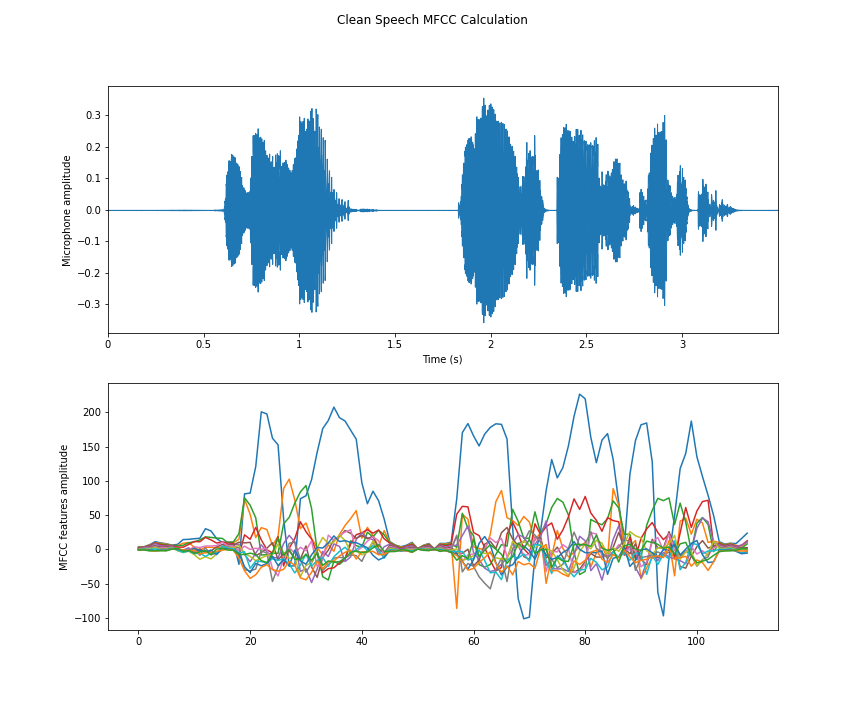
\includegraphics[width=1\textwidth]{thesistemplate/fig/mfcc_timeseries_comp.png}
    \caption{Normalized audio signal and the first 15 MFCC features for a short speech sample, the zeroth MFCC excluded from the plot.}
    \label{fig:mfcc_time_comp}
  \end{center}
\end{figure}

Research shows that it is viable to feed the time series data directly to a deep recurrent neural network for voice activity detection purposes, although it requires a significantly more complicated network structure, therefore higher computational and memory needs. Given our low-performance microcontroller target, striving for the most efficient implementation is key for real-time inference. Optimized Fast Fourier Transformation (FFT) algorithms are widely available for this purpose for most ARM platforms.

The feature extraction and the following section on neural network training have been conducted in python, which is the most popular and well-supported platform for neural network development. MFCC and most audio-related data manipulations utilized the rich functionalities of multiple python packages, most importantly Librosa and NumPy. Librosa \cite{librosa} is one of the most widely used libraries for audio manipulation and analysis, while NumPy \cite{harris2020NumPy} is a general-purpose library for array manipulation and efficient numeric computations.



\begin{figure}[ht!]
  \begin{center}
    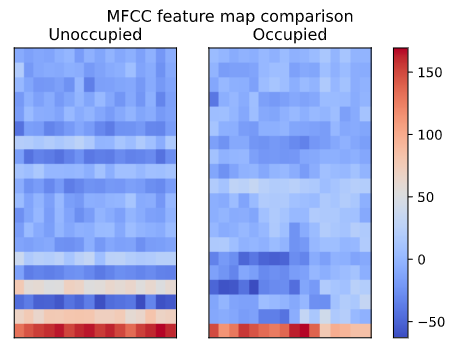
\includegraphics[width=0.6\textwidth]{thesistemplate/fig/mfcc_comp_ex2.png}
    \caption{Comparison of two MFCC image samples from different classes.}
    \label{fig:mfcc_img_comp}
  \end{center}
\end{figure}

Two-dimensional visualization of the dataset after the feature extraction can be seen at \autoref{fig:umap}. Apart from the aesthetic view, data visualization can help to formulate a sense of the problem complexity for classification. The plot can demonstrate the complexity of the problem, given that the task of the learning algorithm is to find the decision boundaries between the clusters of data. The different clusters with the same color show the similarity between elements computed from the same datasource but the clear difference between different sources. The UMAP algorithm \cite{2018arXivUMAP} reduced the 320 dimension input image (20$\times$16) to a two-dimensional representation aiming to preserve the relative differences between elements.



\begin{figure}[ht]
  \begin{center}
    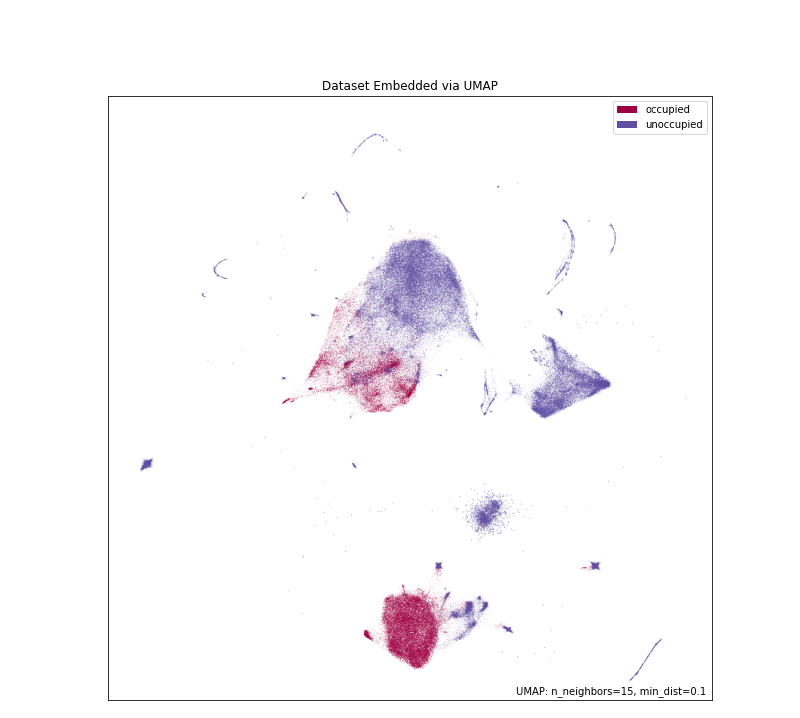
\includegraphics[width=0.8\textwidth]{thesistemplate/fig/umap.png}
    \caption{Visualization of the audio dataset with dimension reduction using UMAP (Uniform Manifold Approximation and Projection \cite{2018arXivUMAP}).  }
    \label{fig:umap}
  \end{center}
\end{figure}


\section{Neural Network design}

The input of the network is fixed to a 20 by 16 two-dimensional matrix of MFCC features, representing 500 ms of audio, while the output is the classification probability for the two classes, occupied and unoccupied room. Labels for all the training data are assigned, making it a fully supervised machine learning problem. Data representing occupied meeting room has 1, unoccupied 0 as a label, which simplifies the calculation of the loss function. The model therefore will have a fixed input size of 20$\times$16 with 2 output nodes each representing the prediction probability that a given input belongs to one of the predefined classes. 

Following a common practice in Data science, the whole dataset was first divided up into three subsets, training, validation, and test set, with ratios of 70\%, 15\%, and 15\% respectively.


Due to limitations of the target hardware and lack of software library support for embedded systems, this work restricts the network structure experiments to feed-forward neural networks only by using fully-connected and convolutional layers as main building blocks and discards more advanced methods such as transformers or recurrent neural networks in general. Recurrent neural networks have the advantage to encapsulate temporal information of the data flow although it usually generates harder training problems and slower convergence. Aggregating the features for longer and then feed them to the network is an alternative to preserve at least partially the temporal characteristics of the input signal at the expense of additional delay. Taking this compromise will allow us to develop solutions based on convolution and linear transformation layers, which efficient implementation exists for most microcontroller platforms.

Additionally, the machine learning framework has to be chosen carefully, given that at some point after the training the models need to be transferred to most probably an Embedded C environment, which might raise some compatibility issues or complicates the prototyping process unnecessarily. The development started with PyTorch \cite{NEURIPS2019Pytorch} but during the first early tests, we have faced great difficulty using the saved model file or converting it to other formats such as ONNX (Open Neural Network Exchange) \cite{bai2019onnx} without success. Unfortunately, at the time of this thesis Embedded machine learning as a field is still in an immature early state and most libraries provide only limited functionality. Although looking for alternatives again now from an embedded inference point of view TensorFlow \cite{tensorflow2015-whitepaper} has made a significant amount of effort to enable the embedded application of their well-established platform. TensorFlow Lite and TensorFlow Lite for Microcontrollers are their solutions for mobile and IoT edge devices for on-device inference. Moreover, Tensorflow Keras \cite{chollet2015keras} provides a simple API interface for most functionality of the TensorFlow framework, therefore in the next sections we will use Keras exclusively as the main Python library for implementing various models.

During the experimentation step for the best neural network architecture and hyperparameter tuning, our main objectives were the highest accuracy on the test set with the least network parameters needed. Tests showed that the number of parameters in the network is directly correlated to the amount of computation i.e. floating number operations (FLOPs) required to run the inference. This is an important observation since our target platform is limited both in memory and CPU power. 

\section{Model architecture optimization}

Finding the best possible layer structure and hyperparameter settings can be highly challenging even for simple problems given the high dimensionality of the optimization, the multimodality of the loss function, and the inherent randomness of the training process. Starting with the same parameters the outcome could be radically different for multiple runs. Considering the high-dimensional search space we needed to make educated guesses on the importance of the different aspects of the training, focusing on a few key metrics while keeping other less relevant details in the same setting. The model optimization had been conducted in multiple exhaustive grid search manners, mostly looking for the best architectural choices but also examining the effect of multiple training setup options.

All the training experiments shared a few properties. Categorical cross-entropy loss was used to measure the performance of the model, and the basis for adjusting the parameters automatically based on the discrepancy using backpropagation and Adam optimizer. The initial learning rate was set to 5e-4 with a batch size of 512. ReLU activation function was selected for all occasions except for the last layer where the Softmax function was applied. The Softmax function takes the input tensor and rescales it that each element will lie in between zero and one and the sum of the values add up to one. Thus the network output can be treated as a probability distribution over the predicted classes, which makes it ideal for comparing the output with the target labels using cross-entropy loss.


\begin{equation}
    Softmax(x_i) = \frac{\exp(x_i)}{\sum_{j}^{ }\exp(x_j))}
\end{equation}

The number of epochs was set to four in all tests to allow fair comparison between the different models. One epoch means one iteration through the entire training set during the training process. The relatively low epoch number was selected in a heuristic manner, models with more epochs were prone to overfitting or predicting constantly one of the labels in real-time testing. The good results even with such a low number of epochs are feasible only because of the small network architectures with a few tens of thousands of parameters and fairly simple problem definition with the constructed dataset.

There were two testing measures applied, and during the experimentation both of them will be reported on the graphs. The first is the traditional prediction accuracy performed on the test set and the second is the result of a short Voice Activity Detection test simulated with short new recordings from the target microphone directly. The new test samples were labeled with the Google WebRTC VAD implementation, and the model performance was measured against those labels. The test audio file takes only a few minutes and was recorded with one speaker in a low background noise environment. It is relatively easy to detect presence even just looking at the raw audio signal but it turned to be useful to test the models also in this way since many of the test cases performed well on the test dataset but produced many unexpected mostly false-positive predictions during the real-world test. The introduction of this audio test shortened the testing process by a significant amount and gave a great tool for detecting overfitting.

\begin{figure}[ht]
  \begin{center}
    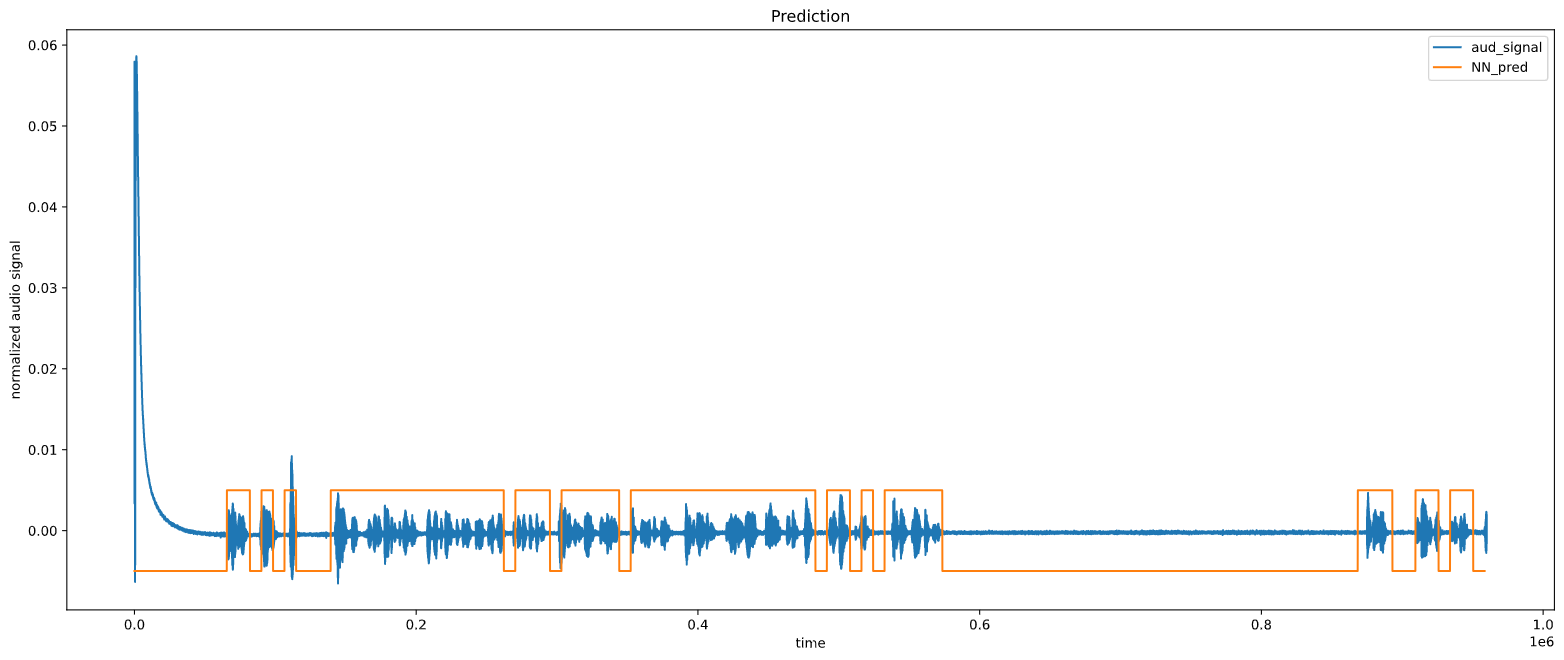
\includegraphics[width=1\textwidth]{thesistemplate/fig/signal_and_pred.png}
    \caption{Correctly functioning model prediction output with clean speech signal.}
    \label{fig:wave_and_pred}
  \end{center}
\end{figure}



\subsection{Fully Connected Neural Network experiments}

The overall structure of the fully connected networks presented in this thesis is summarised at \autoref{fig:FC_structure} below. The custom-developed flexible Python class definition allows us to generate models with different properties while keeping the same structure. Batch Normalization layers can be switched on or off altogether, while the effect of Dropout layers can be regulated with the dropout rate values between 0 and 1. Providing 0 as a probability will change the layer to identity transformation, leaving all the input values intact and forwarding it to the next layer. In most cases when dropout was used the ratio was set to 50\%.

The model architecture starts with the application of a Flatten layer, which was necessary to transform the two-dimensional input to only a list of numbers since the Linear layer only accepts one-dimensional input. This step will make the FCN and CNN models fully compatible and interchangeable, given that their input and output shapes are matching.

The relative position of the Batch Normalization layer in the network varies in recent research. The original Batch Normalization paper \cite{ioffe2015batch} and the first ResNet \cite{he2015deep_resnet} architecture suggest to place the BN layer between the linear and ReLU layers (Conv, BN, ReLU) to maximise the effect of the activation function, where ResNet-v2 paper \cite{he2016identity_resnet_v2} propose alternatives where in some situation BN after the activation function (Conv, ReLU, BN) also lead to improved results in different circumstances. After a few trials, the first arrangement of layers provided a more stable training result, therefore that part will be fixed throughout the experimentation.
% https://forums.fast.ai/t/where-should-i-place-the-batch-normalization-layer-s/56825/4
% and  Gülçehre \& Bengio \cite{ghre2013knowledge_bn_after_relu}


The number of classifier blocks is a configurable property of the model, moreover, the width of each linear layer (the number of neurons)  inside a block is a free parameter too. The only fixed linear layer is the last one called Head in the image with two neurons. This is to ensure compatibility with the labeling of the training data, one for each class. However, since linear layers have significantly larger parameter requirements than Convolutional layers, it limits its usability if not designed carefully. \autoref{fig:FC_1layer} demonstrates that even one wide layer of 512 neurons used after the input has a parameter need around 160000 floating-point numbers which exceeds 1MB of model size when saved. In the Supervised machine learning training context it is not rare to have models taking up multiple gigabytes of space, but in our case, larger models restrict the embedded platform options by a large amount or force to select an unnecessary expensive device for the purpose.


\begin{figure}[ht!]
  \begin{center}
    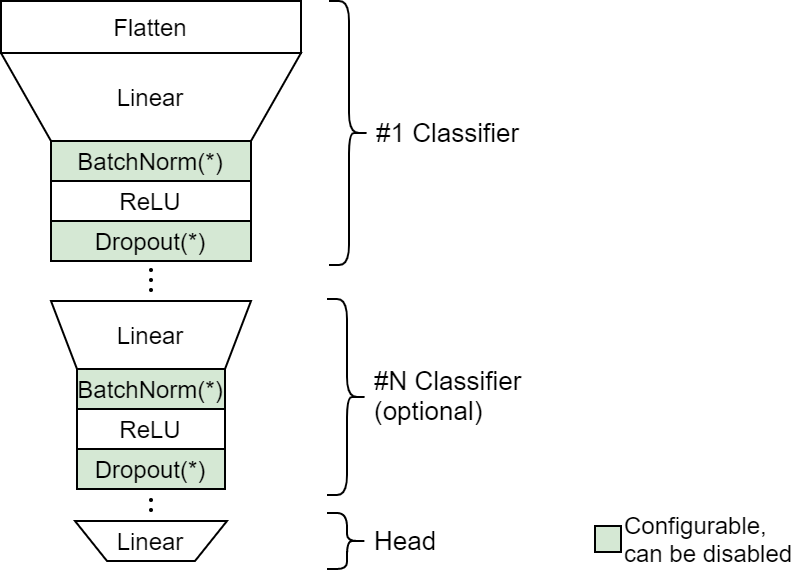
\includegraphics[width=0.7\textwidth]{thesistemplate/images/nn_layer_st_fcn.png}
    \caption{Flexible Fully Connected Network layer structure, additional classifier blocks can extend the model, Batch Normalization and Dropout layers can be turned off.}
    \label{fig:FC_structure}
  \end{center}
\end{figure}


The model names visible in graphs are coding the architectural choices for ease of identification. The layout follows a predefined pattern:

\begin{equation*}
FC\_L\{layers\}\_\{layer\_sturct\}\_\{DR\}\_\{BN\}
\end{equation*}


\begin{table}[h!]
\begin{tabular}{l|l}
\textbf{Label}      & \textbf{Description}  \\
\hline
$layers$     & Number of Fully Connected layers \\
$layer\_struct$ & Structure of linear classifier, multilayer allowed \\
$DR$         & Dropout applied           \\
$BN$         & Batch Normalization applied           
\end{tabular}
\caption{FCN model naming convention.}
\end{table}


where $layers$ denote the number of linear layers the model has excluding the Head, $layer\_sturct$ the number of neurons in each linear layer, and lastly $DR$ and $BN$ act as a flag indicating the presence of Dropout and Batch Normalization layers.

A generated two-layer fully connected network layer structure is demonstrated at \autoref{tab:FC_2layer}. This example network has both Batch Normalization and Dropout features implemented. As the table shows most of the parameters are dedicated to the first linear layer because the first layer has the most input and output nodes which determines the weights matrix (320$\times$128 for the weights plus an additional 128 for the bias terms).

\begin{table}[h]
\centering
\begin{tabular}{lllr}
\hline
\textbf{Layer} & \textbf{Type}  & \textbf{Params} & \textbf{Output shape} \\
\hline
0     & Flatten              & 0      & (1, 320)     \\
1     & Linear               & 41088  & (1, 128)     \\
2     & Batch\_normalization & 512    & (1, 128)     \\
3     & Activation (ReLU)    & 0      & (1, 128)     \\
4     & Dropout              & 0      & (1, 128)     \\
5     & Linear               & 4128   & (1, 32)      \\
6     & Batch\_normalization & 128    & (1, 32)      \\
7     & Activation (ReLU)    & 0      & (1, 32)      \\
8     & Dropout              & 0      & (1, 32)      \\
9     & Linear               & 66     & (1, 2) \\
% Total params: 45,922
\hline
\end{tabular}
\caption{Layer structure and number of parameters per layer for a two layer Fully Connected Network with Dropout and BN (FC\_L2\_128-32\_DR\_BN). }
\label{tab:FC_2layer}
\end{table}


\subsubsection{Test with one linear layer}

The first grid search aims to provide an overall view of the classification complexity using only one fully connected layer with three different width sizes, 128, 256, and 512. At the same time, the effect of Batch Normalization and Dropout layers are also tested. This four combination, on or off for both layers and together with the three layer width option it gives a total of 12 cases. The network test accuracy values are plotted in \autoref{fig:FC_1layer}.

As it was described in the previous section there were two accuracy measures assigned for each trained model. The first marked with blue here and in the next experiments too is related to the prediction accuracy on the test set, while the orange accuracy measures are representing the model performance on a selected voice recording from the actual microphone. The second test is trying to simulate the deployed model behavior on embedded, and as we can see on the graph the results are significantly different in some cases as a sign of overfitting. In those low accuracy scenarios, around 50\%, the model prediction was mostly constant during the test, which was still correct half of the time, given the test file characteristic. The big difference in these two testing scenarios can be the consequence of using external data sources for training and having a relatively low proportion of actual recorded audio.

Having only one layer of nodes without any regularization resulted in poor performance generally, while the introduction of BN or Dropout increased the test accuracy significantly and the best results were achieved using both, regardless of the fully connected layer width. Although a slight increase in accuracy is achieved by using wider networks in the best BN DR combinations, but the number of parameters required is two and four times more than the 128 nodes version. Given that our objective is also to minimize the memory footprint of the model for efficiency reasons we will narrow down the search space where the number of parameters is less than 100 000, and from closely identical accuracy values will choose the one with fewer parameters.


From this test FC\_L1\_128\_DR\_BN and FC\_L1\_256\_DR\_BN architectures were selected for the final comparison.
\begin{figure}[ht!]
  \begin{center}
    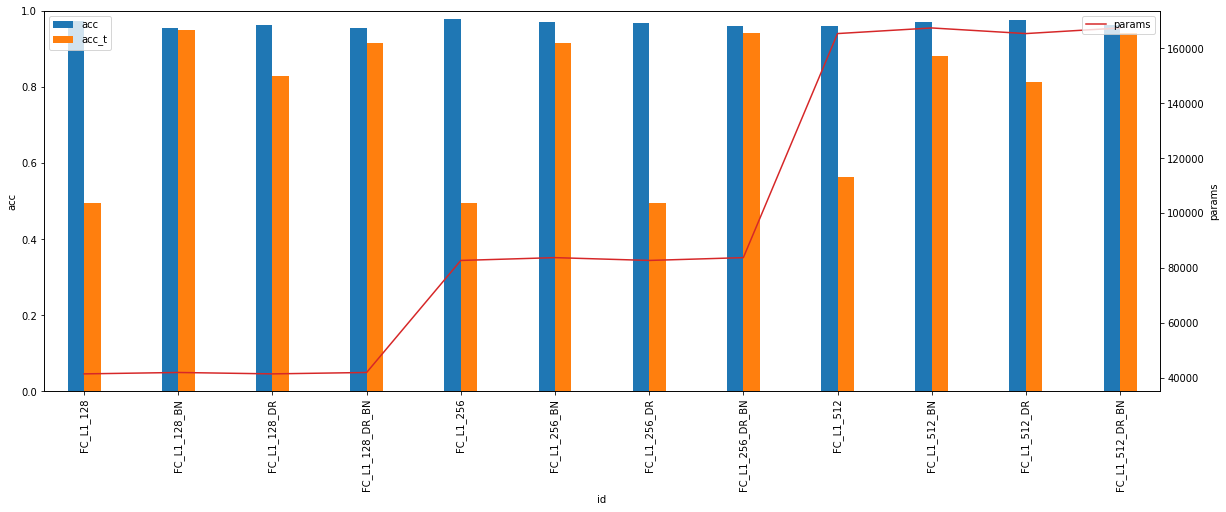
\includegraphics[width=1\textwidth]{thesistemplate/fig/fc_1layer_plot.png}
    \caption{One layer fully connected structure test, number of parameters in red line, number of nodes varied, while testing Dropout and BN. (Columns are: acc - accuracy on the test set, acc\_t - prediction accuracy on a custom speech recording from the mic used in the implementation.) }
    \label{fig:FC_1layer}
  \end{center}
\end{figure}

\subsubsection{Test with two linear layers}

The second experiment with FCN will focus on minimizing the number of parameters by adding another additional layer to a narrower first layer, hoping to maintain model generalizability even with smaller memory needs. The models consist of 128-32, 256-32, 64-16 node structures. As before the effect of Batch Normalization and Dropout was tested on every architectural choice.

The test results are reported at \autoref{fig:FC_2layer}. Similar to the first experiment the combination of both BN and DR lead to the highest accuracy most stable and reproducible results among the test cases. The lack of DR caused model overfitting in most cases, and the effect is visible when it was tested with the custom voice recording. And as the two rightmost models on the figure demonstrate, high-performing models can be trained even using as low as 20 thousand parameters with a carefully chosen architecture.

\begin{figure}[ht!]
  \begin{center}
    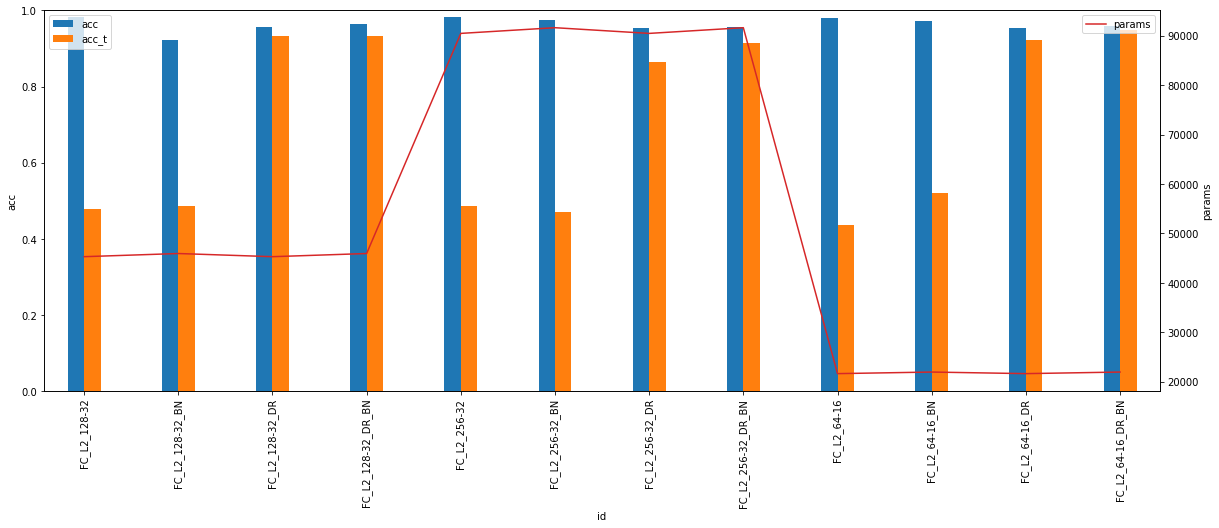
\includegraphics[width=1\textwidth]{thesistemplate/fig/test_fc_2lay_plot.png}
    \caption{Two layers of fully connected layer structure test, number of parameters in red line, number of nodes varied, effect of Dropout and BN. (Columns are: acc - accuracy on the test set, acc\_t - prediction accuracy on a custom speech recording from the mic used in the implementation.)}
    \label{fig:FC_2layer}
  \end{center}
\end{figure}

\subsubsection{Test with different dropout values}

In the last FCN based grid search training, the effect of different dropout rates (0, 0.25, 0.5) was tested with the combination of BN layers. Zero dropout rate means no dropout or identity function from an implementation point of view.

The test result reported at \autoref{fig:FC_2layer_small}. Models without dropout lead to overfitting and selecting smaller values such as 0.25 also does not help to reduce the effect on the second test set. However 50\% dropout rate have been proven to be sufficient for mitigating the model limitations and enabled good response on both test sets.

\begin{figure}[ht!]
  \begin{center}
    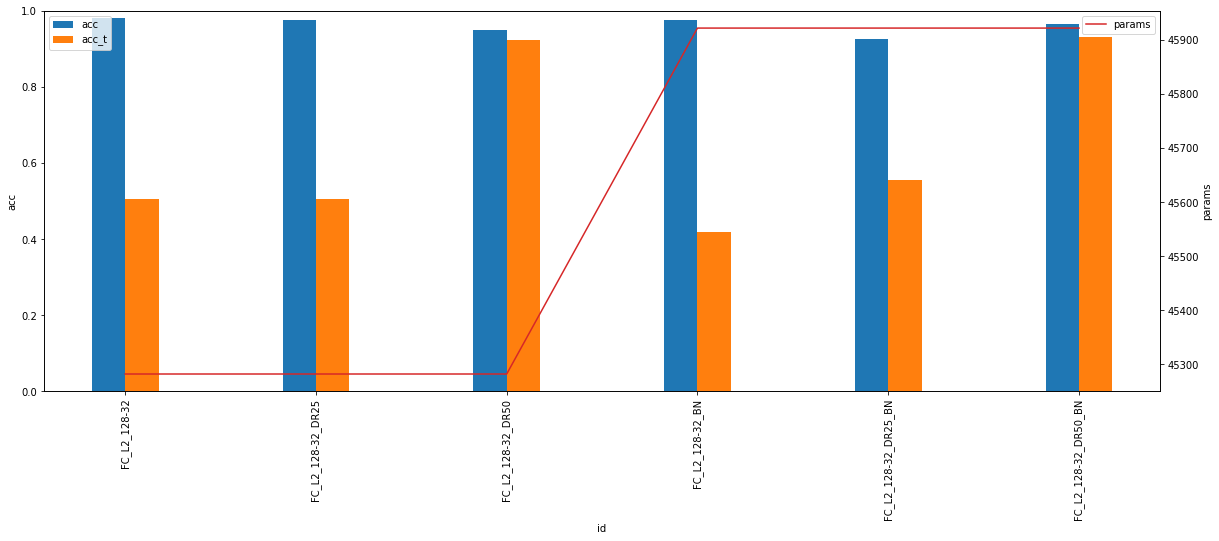
\includegraphics[width=1\textwidth]{thesistemplate/fig/test_fc_2lay_smalll_plot.png}
    \caption{The effect of different Dropout values (0, 0.25, 0.5) and Batch Normalization combined for the selected two layer Fully connected network.  (Columns are: acc - accuracy on the test set, acc\_t - prediction accuracy on a custom speech recording from the mic used in the implementation.)}
    \label{fig:FC_2layer_small}
  \end{center}
\end{figure}

\newpage
\subsection{Convolutional Neural Network experiments}

Constructing Convolutional Neural Networks applied the same principles as described in the previous FCN experimentation section. The architectural model schema is summarised in \autoref{fig:CNN_structure}. The three main parts are the Feature extractor the Classifier and the Head of the network. The feature extractor module consists of 2D Convolution, Batch Normalization, RelU Activation, and Max pooling. The position of the BN layer is between the convolution and the activation function as it was in the FCN networks and the BN paper \cite{ioffe2015batch}. The 2D Max pooling layer downsamples the input by a factor of two, by selecting the maximal value in each two-by-two pool frame size. Multiple feature extractors can be stacked after each other, and after that, a fully connected layer based Classifier comes. The Classifier can be configured to have multiple linear layers with arbitrary width and using or not the Dropout layer after the ReLU activation. The Dropout rate is kept to 50\% when it is used. Batch Normalization layers can be switched on and off in the Feature extractors by a parameter similarly. The Head module consists only of a linear layer as in the FCN case outputting probability values for each class.

\vspace{100px}

\begin{figure}[h!]
  \begin{center}
    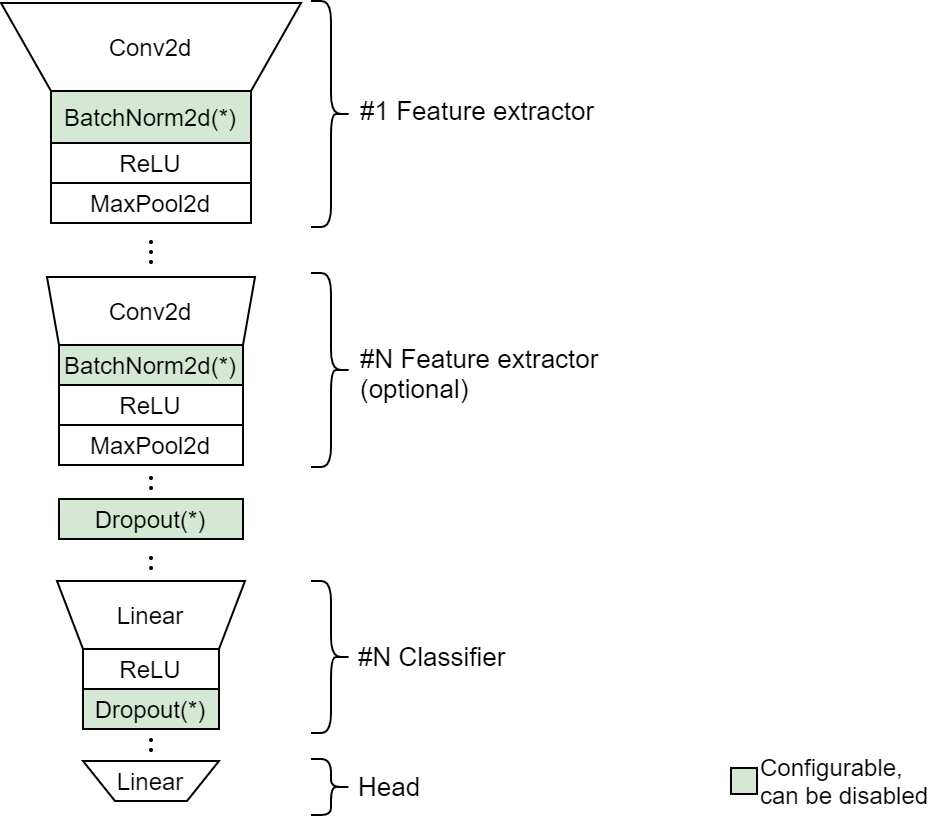
\includegraphics[width=0.7\textwidth]{thesistemplate/images/nn_layer_st_cnn.png}
    \caption{Flexible CNN model architecture, the number of Feature extractor and Classifier blocks can be altered, Batch Normalization and Dropout layers can be turned off.}
    \label{fig:CNN_structure}
  \end{center}
\end{figure}

CNN saved models follow a predefined naming convention to ease the archiving and logging process:

\begin{equation*}
CNN\_L\{layers\}\_K\{kernel\}\_F\{filters\}\_\{fc\_layers\}\_\{DR\}\_\{BN\}
\end{equation*}

\begin{table}[h!]
\begin{tabular}{l|l}
\textbf{Label}      & \textbf{Description}  \\
\hline
$layers$     & Number of Convolutional layers (Feature extractors) \\
$kernel$     & Size of the 2D convolution kernel \\
$filters$    & Number of filters learned in each Conv layer     \\
$fc\_layers$ & Structure of linear classifier, multilayer allowed \\
$DR$         & Dropout applied           \\
$BN$         & Batch Normalization applied           
\end{tabular}
\caption{CNN model naming convention.}
\end{table}

\begin{table}[h]
\centering
\begin{tabular}{lllr}
\hline
\textbf{Layer} & \textbf{Type}  & \textbf{Params} & \textbf{Output shape} \\
\hline
0     & Conv2D                      & 80     & (1, 18, 14, 8) \\
1     & BatchNormalization        & 32     & (1, 18, 14, 8) \\
2     & Activation (ReLU)           & 0      & (1, 18, 14, 8) \\
3     & MaxPooling                  & 0      & (1, 9, 7, 8)   \\
4     & Dropout                     & 0      & (1, 9, 7, 8)   \\
5     & Conv2D                      & 584    & (1, 7, 5, 8)   \\
6     & BatchNormalization        & 32     & (1, 7, 5, 8)   \\
7     & Activation (ReLU)           & 0      & (1, 7, 5, 8)   \\
8     & MaxPooling                  & 0      & (1, 3, 2, 8)   \\
9     & Dropout                     & 0      & (1, 3, 2, 8)   \\
10    & Flatten                     & 0      & (1, 48)        \\
11    & Linear                      & 6272   & (1, 128)       \\
12    & Dropout                     & 0      & (1, 128)       \\
13    & Linear                      & 4128   & (1, 32)        \\
14    & Dropout                     & 0      & (1, 32)        \\
15    & Linear                      & 66     & (1, 2)        \\ 
\hline
% Total params: 45922
\end{tabular}
\caption{Layer structure and number of parameters per layer for a two layer CNN with dropout and batch normalization, 8 filters, kernel size of 3$\times$3 classifier shape [128, 32] (CNN\_L2\_K3\_F8\_128-32\_DR\_BN). }
\end{table}




\subsubsection{Test for number of filters, filter size}


In the first test, visible on \autoref{fig:CNN_1layer}, the classifier shape was kept at constant 64 nodes, while the number of filters was varied in four different levels 2, 4, 8, and 16. Batch normalization and Dropout layers were altered in each case, providing a total of 16 combinations. Examining the accuracy results, overall, more filters usually resulted in better performance but there is no clear improvement by introducing significantly more filters to the model. Therefore a smaller structure K3\_F4, kernel size of 3$\times$3, and 4 learned filters are selected for further investigation.

\begin{figure}[ht!]
  \begin{center}
    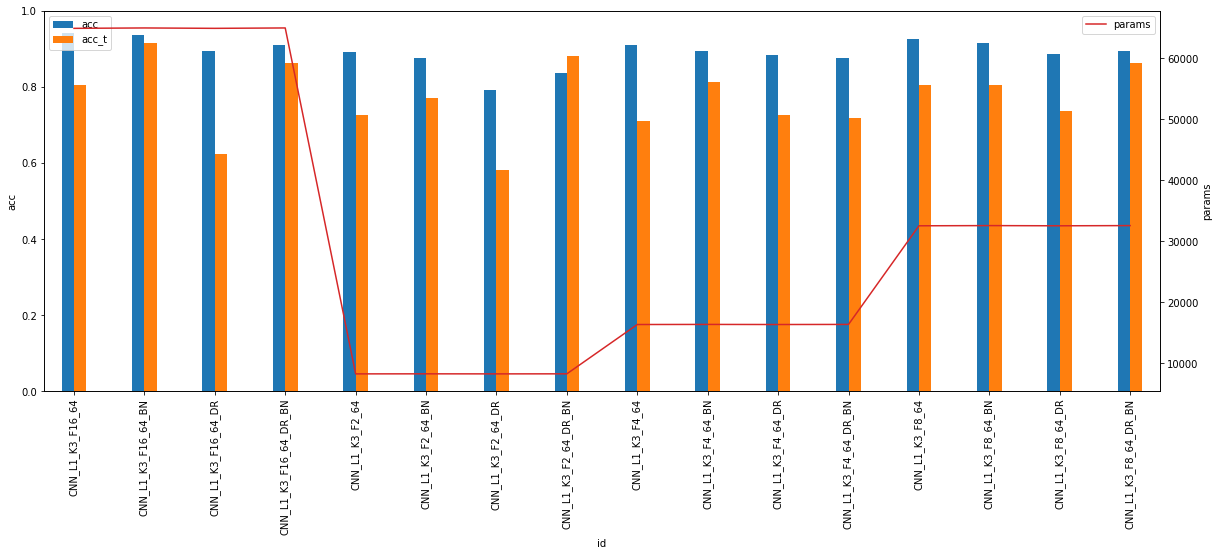
\includegraphics[width=1\textwidth]{thesistemplate/fig/test_cnn_1lay_plot.png}
    \caption{Number of filters does not really improve the accuracy, although it has a great impact in the total number of parameters. Usage of Batch Normalization and Dropout layers does not show significant improvements in this test. (Columns are: acc - accuracy on the test set, acc\_t - prediction accuracy on a custom speech recording from the mic used in the implementation.)}
    \label{fig:CNN_1layer}
  \end{center}
\end{figure}


\subsubsection{Test for one layer classifier with different width}

For the second experiment, we have varied the classifier size while keeping the feature extractor with kernel size 3$\times$3 and 4 filters. The accuracy results are reported at \autoref{fig:CNN_1lclassf}. Versions with dropout performed lower than the competition on average and using BN exclusively produced the best results. 

\begin{figure}[h!]
  \begin{center}
    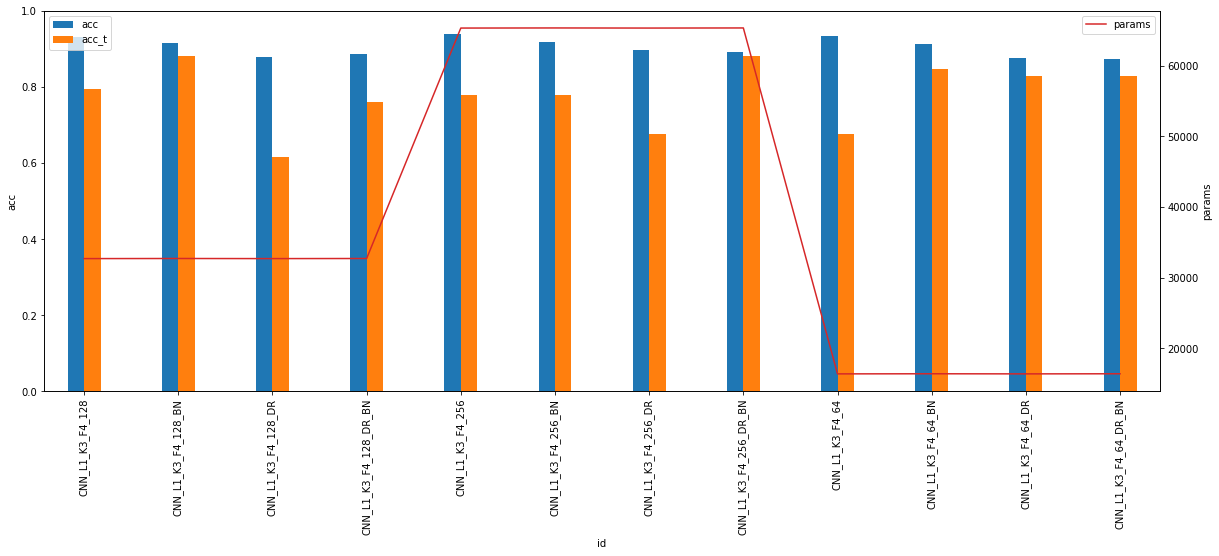
\includegraphics[width=1\textwidth]{thesistemplate/fig/test_cnn_clss_plot.png}
    \caption{One layer classifier different node sizes, BN, DR. (Columns are: acc - accuracy on the test set, acc\_t - prediction accuracy on a custom speech recording from the mic used in the implementation.)}
    \label{fig:CNN_1lclassf}
  \end{center}
\end{figure}


\subsubsection{Test for two layer classifier with different width}

In the last test, the effect of an additional fully connected layer in the classifier will be examined. Batch normalization is used without dropout, the only variation across the models is the classifier shape. Result are reported at \autoref{fig:CNN_classf}.

\begin{figure}[h!]
  \begin{center}
    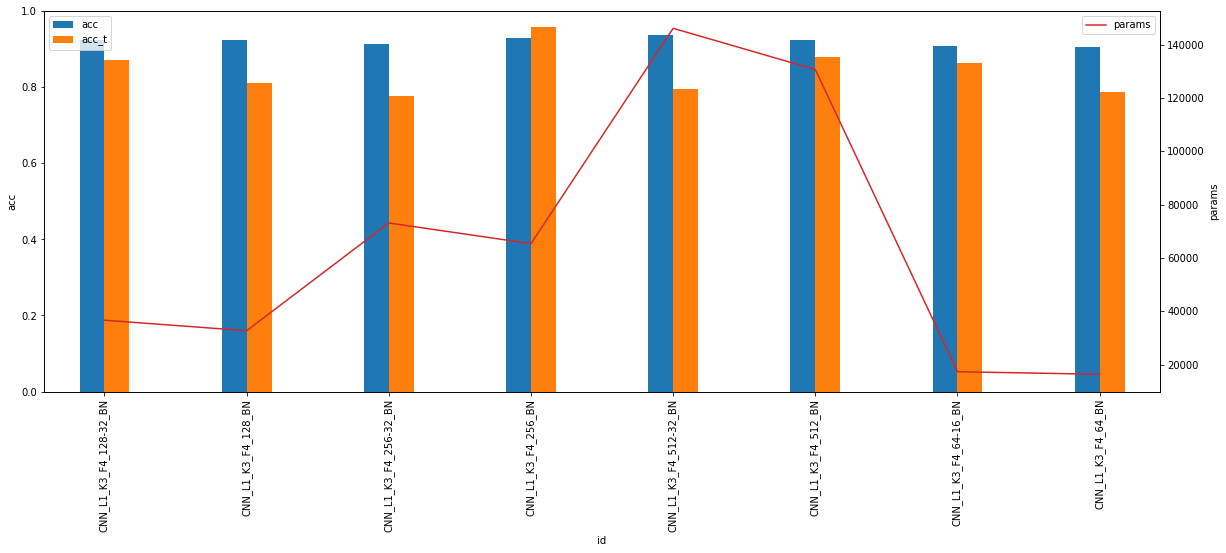
\includegraphics[width=1\textwidth]{thesistemplate/fig/test_cnn_clss2_plot.png}
    \caption{Experiment on one or two fully connected layer in the classifier while using Batch normalization. (Columns are: acc - accuracy on the test set, acc\_t - prediction accuracy on a custom speech recording from the mic used in the implementation.)}
    \label{fig:CNN_classf}
  \end{center}
\end{figure}




\section{Model selection for embedded implementation}

For the embedded study, four models were selected both from FCN and CNN training. During the selection, the aim was to represent distinctive elements of the search space with the highest accuracy values and least false-positive rates. All the four Fully-connected models utilize both Batch Normalization and Dropout layers, the main difference is in the number of layers and their width. Choosing only bigger networks might be a limiting factor computationally given the selected hardware components.

Among trained CNN models, all of the selected ones apply Batch Normalization and one also with Dropout. The main differentiator is in the classifier structure mainly, using one or two Fully-connected layers and smaller or bigger node sizes per layer.
\newline

% FCN models for embedded test (one layer small/large, two layers small/large):

% \begin{itemize}
%     \item[$-$] 1 layer, 128 nodes, DR, BN
%     \item[$-$] 1 layer, 256 nodes, DR, BN
%     \item[$-$] 2 layers, 64-16, DR, BN
%     \item[$-$] 2 layers, 128-32, DR, BN
% \end{itemize}


\begin{table}[h!]
\begin{tabular}{|l|l|l|l|}
\hline
\textbf{Name}                   &  \textbf{Node structure} & \textbf{Dropout} & \textbf{Batch Norm.} \\ \hline
FC\_L1\_128\_DR\_BN    & 128            & Yes     & Yes                 \\ \hline
FC\_L1\_256\_DR\_BN    & 256            & Yes     & Yes                 \\ \hline
FC\_L2\_64-16\_DR\_BN & 64-16          & Yes     & Yes                 \\ \hline
FC\_L2\_128-32\_DR\_BN  & 128-32         & Yes     & Yes                 \\ \hline
\end{tabular}
\caption{Selected Fully Connected Network model structures.}
\end{table}


\begin{table}[h!]
\begin{tabular}{|l|l|l|l|l|l|}
\hline
\textbf{Name}                        & \textbf{Kernel} &\textbf{Classifier}  & \textbf{Dropout} & \textbf{BN} \\ \hline
CNN\_L1\_K5\_F4\_64\_DR\_BN &  5$\times$5           & 64                        & Yes     & Yes                 \\ \hline
CNN\_L1\_K3\_F4\_256\_BN    &  3$\times$3           & 256                       & No      & Yes                 \\ \hline
CNN\_L1\_K3\_F4\_64-16\_BN  &  3$\times$3           & 64-16                     & No      & Yes                 \\ \hline
CNN\_L1\_K3\_F4\_128-32\_BN &  3$\times$3           & 128-32                    & No      & Yes                 \\ \hline
\end{tabular}
\caption{Selected Convolutional Neural Network model structures, BN - Batch Normalization.}
\end{table}

% CNN models for embedded test (one layer small/large, two layers small/large):
% \begin{itemize}
%     \item 1 layer, 64 nodes, DR, BN
%     \item 1 layer, 256 nodes, BN 
%     \item 1 layer, 64-16 nodes, BN
%     \item 1 layer, 128-32 nodes, BN
% \end{itemize}



% FCN:
% FC_L1_128_DR_BN  - test_fc_1lay
% FC_L1_256_DR_BN  - test_fc_1lay
% FC_L2_128-32_DR50_BN - test_fc_2lay_small
% FC_L2_64-16_DR_BN - test_fc2lay

% CNN
% CNN_L1_K5_F4_64_DR_BN - the one, (second working model)
% CNN_L1_K3_F4_256_BN   - test_cnn_clss
% CNN_L1_K3_F4_64-16_BN - test_cnn_clss2
% CNN_L1_K3_F4_128-32_BN - test_cnn_clss2













%----------------------------------------
%
% Alternative table for audio database


%\begin{table}[ht]
%\centering
%\begin{tabular}[t]{lr}
%\hline
%Type                        & duration\\
%\hline
%\textit{Occupied:}           & \\
%
%Librispeech dev             &  323:16\\
%QUT-Noise home-kitchen      &   33:09\\
%Open office recordings      &   10:00\\
%\hline
%Total:                      &  366:25\\
%\hline
%\\
%\textit{Empty:}              &       \\
%Meeting room recordings     &   43:00\\
%QUT-Noise car-window        &   44:35\\
%White noise                 &   15:00\\
%\hline
%Total:                      &  102:35\\
%\hline
%\end{tabular}
%\caption{Audio Database size}
%\end{table}%
 





% You have now stated your problem, and you are ready to do something
% about it!  \emph{How} are you going to do that? What methods do you
% use?  You also need to review existing literature to justify your
% choices, meaning that why you have chosen the method to be applied in
% your work.

% An example of a traditional LaTeX table
% ------------------------------------------------------------------
% A note on underfull/overfull table cells and tables:
% ------------------------------------------------------------------
% In professional typography, the width of the text in a page is always a lot
% less than the width of the page. If you are accustomed to the (too wide) text
% areas used in Microsoft Word's standard documents, the width of the text in
% this thesis layout may surprise you. However, text in a book needs wide
% margins. Narrow text is easier to read and looks nicer. Longer lines are 
% hard to read, because the start of the next line is harder to locate when
% moving from line to the next. 
% However, tables that are in the middle of the text often would require a wider
% area. By default, LaTeX will complain if you create too wide tables with
% ``overfull'' error messages, and the table will not be positioned properly
% (not centered). If at all possible, try to make the table narrow enough so
% that it fits to the same space as the text (total width = \textwidth).
% If you do need more space, you can either
% 1) ignore the LaTeX warnings 
% 2) use the textpos-package to manually position the table (read the package
%    documentation)
% 3) if you have the table as a PDF document (of correct size, A4), you can use
%    the pdfpages package to include the page. This overrides the margin
%    settings for this page and LaTeX will not complain.
% ------------------------------------------------------------------
% Another note:
% ------------------------------------------------------------------
% If your table fits to \textwidth, but the cells are so narrow that the text
% in p{..}-formatted cells does not flow nicely (you get underfull warnings 
% because LaTeX tries to justify the text in the cells) you can manually set
% the text to unjustified by using the \raggedright command for each cell 
% that you do not want to be justified (see the example below). \raggedleft 
% is also possible, of course...
% ------------------------------------------------------------------
% If you need to have linefeeds (\\) inside a cell, you must create a new
% paragraph-formatting environment inside the cell. Most common ones are 
% the minipage-environment and the \parbox command (see LaTeX documentation
% for details; or just google for ``LaTeX minipage'' and ``LaTeX parbox'').
